% Messwerte: Alle gemessenen Größen tabellarisch darstellen
% Auswertung: Berechnung geforderter Ergebnisse mit Schritten/Fehlerformeln/Erläuterung/Grafik (Programme)
\section{Auswertung}
\label{sec:auswertung}

\subsection{Fehlerrechnung}
\label{sec:Fehlerrechnung}

%\subsection{Formeln für den Mittelwert, den Gauß-Fehler und die Standardabweichung }
%\label{sec:Formeln fuer den Mittelwert, den Gauss-Fehler und die Standardabweichung}
    Für den Mittelwert gilt
    \begin{equation}
    \bar{x} = \frac{1}{N}\sum\limits_{i = 1}^N x_i .
    \end{equation}

    Für den Fehler des Mittelwertes gilt
    \begin{equation}
        \Delta \bar{x}=\frac{1}{\sqrt{N}} \sqrt{\frac{1}{N-1} \sum_{i=1}^N\left(x_i-\bar{x}\right)^2}.
        \end{equation}

    Für die Gaußsche Fehlerfortpflanzung gilt

    \begin{equation}
        \Delta f=\sqrt{\sum_{i=1}^N\left(\frac{\partial f}{\partial x_i}\right)^2 \cdot\left(\Delta x_i\right)^2}.
    \end{equation}

    Diese Formeln werden für sämtliche Fehlerrechnungen in diesem Versuch verwendet, ohne sie für die 
    jeweiligen Rechnungen explizit anzugeben. Die Rechnungen selbst werden dabei mithilfe von
    Uncertainties durchgeführt.

\subsection{Durchlasskurve}
\label{sec:Durchlasskurve}

Zunächst wird die Filterkurve eines Selektivverstärkers untersucht, wobei eine effektive Spannung $U_E$ in Höhe von $ \SI{1}{\volt}$ 
verwendet. Aufgenommen wird dabei die Ausgangspannung $U_A$ in Anhängigkeit von der Frequenz $v$. Die Frequenz wurde von $\SI{2}{\kHz}$ auf 
$\SI{31}{\kHz}$ hochgedreht. In der \autoref{tab:filterkurve} sind die aufgenommen Messwerte aufgetragen.

\begin{table}[H]
    \centering
    \caption{Die Messwerte für Filterkurve}
    \label{tab:filterkurve}
\begin{tabular}{c c}
    \toprule
          $v \, /\,\si{kHz}$ & $U \,/\,\si{v}$ \\
    \midrule
           2 &    0.01 \\
           4 &    0.02 \\
           6 &   0.025 \\
           8 &    0.03 \\
          10 &    0.04 \\
          11 &    0.05 \\
          12 &    0.06 \\
          13 &    0.07 \\
          14 &    0.08 \\
          15 &   0.095 \\
          16 &   0.115 \\
          17 &   0.145 \\
          18 &    0.19 \\
          19 &    0.26 \\
          20 &    0.42 \\
        20.5 &     0.6 \\
          21 &    0.98 \\
        21.1 &     1.2 \\
        21.2 &     1.3 \\
        21.3 &     1.5 \\
        21.4 &    1.85 \\
        21.5 &    2.35 \\
        21.6 &     3.1 \\
        21.7 &       4 \\
        21.8 &     4.4 \\
        21.9 &     3.8 \\
          22 &    2.95 \\
        22.1 &    2.45 \\
        22.2 &    1.85 \\
        22.3 &    1.55 \\
        22.4 &     1.3 \\
        22.5 &    1.15 \\
          23 &    0.68 \\
          25 &   0.265 \\
          27 &    0.17 \\
          29 &   0.125 \\
          31 &    0.1 \\
    \bottomrule
    \end{tabular}
\end{table}

In der \autoref{fig:plot} wird die Durchlasskurve der aufgenommenen Messwerte abgebildet.
Dabei ist der Quotient $\frac{U_A}{U_E}$ gegen die Frequenz $v$ aufgetragen. Anhand des Graphens lässt sich ablesen, dass das 
Maximum bei $\SI{21.8}{kHz}$ liegt mit einer Spannung von $\SI{4.4}{\volt}$. Dieses Maximum ist dann die Durchlassfrequenz.

\begin{figure}[H]
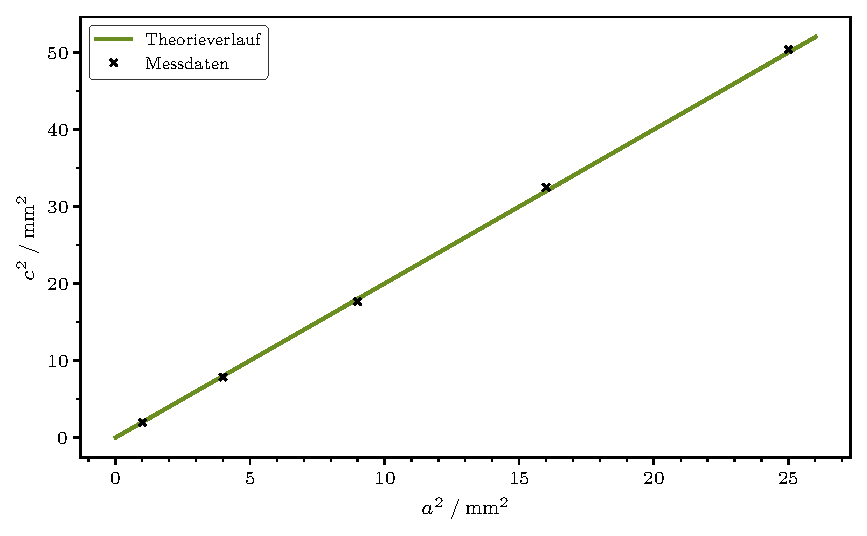
\includegraphics{build/plot.pdf}
	\caption{Filterkurve des Selektivverstärkers mit einer Güte $Q = 20$ und die Ausgleichskurve in Form einer Gaußverteilung .}
	\label{fig:plot}
\end{figure}

\subsection{Suszeptibilität}

\subsection{Effektiver Querschnitt}